\section{Historical Aside on Epidemics}

The history of epidemics is an area whose fascination, in its horrifying nature, crosses the boundaries between science and history. Historically, the most famous epidemics is represented by the Black Death, which, in the 14th century, killed about a third of the European population, which was of 85 million people at the time.\\
One epidemic that has exercised classical scholars for a very long time is the Plague of Athens that occurred in 430BC, the second year of the Peloponnesian War among Athens and Sparta. The Plague has been documented by the Greek Historian Thucydides in his \textit{opera summa} titled \textit{On the Peloponnesian War} (V century BC). Among the illustrious victims of the Plague, there was then Athens' ruler Pericles. According to a 1999 study from the University of Maryland on the nature of that epidemic, the Plague was likely to be typhus, although such claim is still considered controversial among many classical historians.\\
Before proceeding to the main focus of this paper, we provide a brief account of the importance of epidemic models.
First off, we start by acknowledging that there are four main disease-causing microorganisms: viruses, bacteria, parasites and fungi. Models have been implemented to describe the population dynamics of disease agents, as well as the spread of infections, in both their geographical and temporal impact. The practicality of such models relies heavily on the realism put into their implementation. I.e., models do not take into account all possible effects, but they rather incorporate in their mechanisms what appears to be the major components of the issue being studied. Most mathematical models go through several versions before qualitative phenomena can be explained or described with any degree of confidence and epidemics models make no exception. Thus, great care needs to be exercised before making practical use of any epidemic model. Nonetheless, even the simplest model could, and frequently does, raise important points with regards to the underlying dynamics and the possible means of control of the epidemics.\\
These are just a few aspects about the importance of epidemic models.

\subsection{History, Myths and Statistics}
The epidemic of HIV and AIDS has a relative long history of spreading fear, illness and death among populations across the world. However, scientific advances, such as the development of antiretroviral drugs, have enabled people who have access to treatment and medication to endure and live long, healthy lives with HIV.\\
Reportedly, the Human Immunodeficiency Virus (HIV) originated in Kinshasa, the capital and most populated urban area of the Democratic Republic of Congo, around 1920. This was probably a result of the fact that apes and chimps carrying the Simian Immunodeficiency Virus (SIV), a virus closely related related to HIV, were being hunted and eaten by the people living in the area.\\
However, up until 1980, there is no reliable information about the number of people infected with HIV or that had developed AIDS, as HIV was not known and there were no noticeable symptoms to accompany the transmission of the virus. That being said, available data suggests that by 1980 HIV may have already spread to North America, South America, Europe, Africa and Australia. It is believed that in this period, between 100,000 and 300,000 individuals could have been infected.\\
Historically, certain diseases  with a perceived social stigma, or some major socio-economic element attached to, tend to be accompanied by the myth of denial, where scientific conclusions tend to be ignored for ideological reasons. AIDS is one of those diseases.\\
In fact, the term AIDS was only used for the first time in September of 1982 by the United States Center of Disease Control, describing it as "a disease at least moderately predictive of a defect in cell-mediated immunity, occurring in a person with no known case for diminished resistance to that disease"$^{(2)}$.\\
Yet, the major stigma that the disease brought into people's lives, was regarding their sexual tendencies and encounters. For many years, HIV was considered an exclusively homosexual disease and this belief had obviously many sociopolitical consequences when it came down to how to solve the epidemics. The "equation" homosexual encounter = HIV has been a long and threatening stigma on the gay community all across the world and prejudices that rose from it are still very much alive and well even nowadays.\\ 
Arguably, an event that helped moving the conversation forward and, at least partially, away from the aforementioned social stigma, took place on November $7^{th}$ of 1991. In that date then-Los-Angeles-Lakers professional basketball player Ervin "Magic" Johnson announced his seropositivity and consequential retirement from professional sports. This was the second high-profile HIV revelation in the US (actor Rock Hudson had died in 1985 victim of the disease), but it was the first world-known personality to come out with such staggering admission. Ever since, Johnson has spent his life educating young people about the risks of unprotected sexual activities and he is the first major personality to have survived the disease. The same fate was not shared by Rock and Roll legend and Queen's lead singer Freddie Mercury (who admittedly had several homosexual encounters), who announced his seropositivity one week after Johnson did, but died a day later.\\
Regardless of social stigma and the objective problems associated with gathering data on the number of individuals affected, the pattern that characterise the disease needs to be surveilled in order to contain the epidemic. After all, widespread surveillance of human tuberculosis is what eradicated the disease in many developed countries in the 1950's and, for a long time, the lack of knowledge surrounding HIV had created enormous difficulties in designing effective control programmes and related health care facilities. Educating communities, especially women, had proven to be a winning strategy in containing the disease, and yet many of them have repeatedly been blocked by religious establishments (not limited to right fundamentalist Christians). Up until the early 2000's, the lack of surveillance for AIDS had caused major problems in developing effective strategies to contain the epidemics.\\
Many things have changed ever since, and in 2013 the Joint United Programs on HIV/AIDS (UNAIDS) announced that AIDS-related death had fallen 30\% worldwide, after their peak in 2005. Yet, in the US alone, there were an estimated 37,600 new HIV infections in 2014 (most recent available data), according to the CDC database. And, although it is actually statistically accurate to say that homosexuals and bisexual males constitute the greatest risk group with an estimated 26,000 of these new cases, the burden of HIV is not sustained by the gay community alone.
\begin{figure}[H]
	\subfigure[Data from CDC]{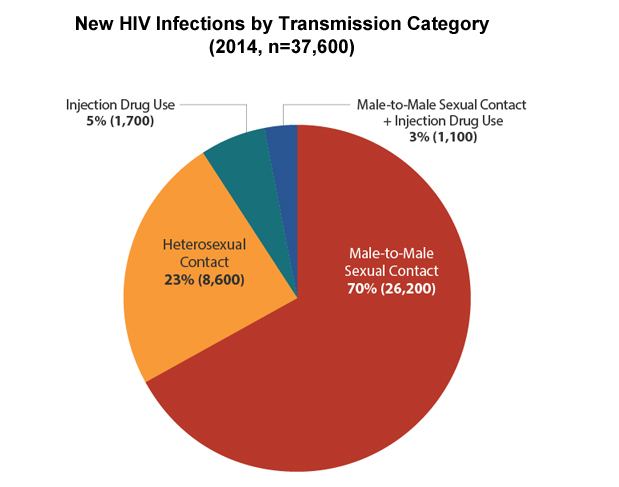
\includegraphics[scale=0.65]{AIDS_sexual.jpg}}	
\end{figure}
\clearpage
\begin{figure}
	\subfigure[Data from CDC]{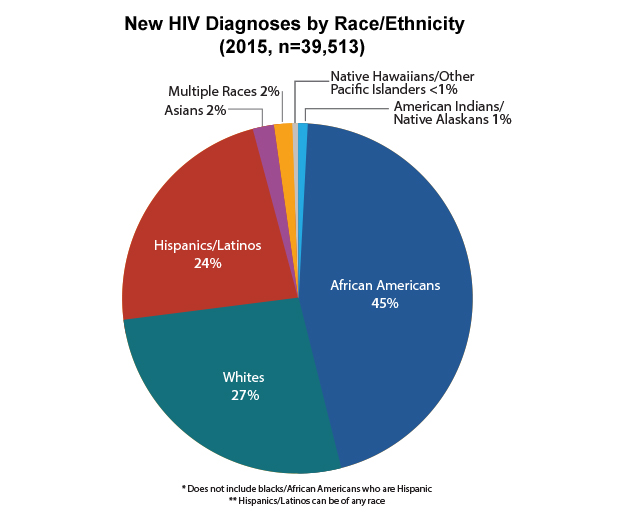
\includegraphics[scale=0.65]{AIDS_ethnic.jpg}}
\end{figure}
Despite scientific progress in medical treatment and countless awareness campaigns, HIV remains a constant and present cause of death. In the United States, in 2014 alone, 6,721 people died from the disease, which was the 8th leading cause of death for individuals aged 25-34, according to the CDC. Worldwide, there were about 1.8 million new cases of HIV in 2016 (most recent available data), with Sub-Saharan Africa accounting for about 64\% of those. There are an estimated 36.7 million individuals living with HIV worldwide, 90\% of whom receive treatment in the form of antiretroviral therapy (ART). Still, of the grand total, about 1 million died in 2016 alone from AIDS-related illnesses.\\

\subsection{Human Immunodeficiency Virus (HIV) - Background on the biology}
HIV is a retrovirus that leads to acquired immune deficiency syndrome, AIDS. Like most of the viruses belonging to the family of \textit{Retroviridae}, HIV only replicates in dividing cells. However, the Human Immunodeficiency Virus has some unique properties even within its family; for instance, it uses the mRNA processing of the cell that invades to synthetize its own viral RNA. Although it had been shown that the dynamics of viral replication is very high \textit{in Vivo} (Ho et al. 1995), the immune system can counteract this replication from 5 to 10 years, depending on the initial infection, sometimes even longer.\\
Infection by the most common variety of the virus, HIV-1, has many complex characteristics that are still not quite completely understood. For instance, the fact that the disease progression can last more than 10 years after the first day of infection; or the fact that immune response only briefly control it, while most viral infections would be eliminated by it. HIV attacks the immune system, primarily infecting CD4-T-cells, a particular class of white blood cells, but also dendritic cells, which play a crucial role in the generation and regulation of adaptive immunity. The T-cell count is normally 500-1500 cells per $\mu$L of blood and, if it drops to 200/$\mu$L or below, then a person is diagnosed with having AIDS. \\
Yet, the CD4 T-cell count is not the only factor used to make a diagnosis on that matter. The Center for Disease Control applies very specific and regularly-updated categories, which include several diseases as symptoms or indicators, that the CDC uses for surveillance purposes. For instance, if a patient with the virus has a T-cell count greater than 500/$\mu$L, but has one of a variety of diseases (from peripheral neuropathy to a recurrent bacteria-pneumonia), then a formal diagnosis is made. The reason for the fall of T-cells is still unknown, but what can be said with confidence is that, because of the central role of CD4 T-cells in immune regulation, their depletion has widespread deleterious effects on the proper functioning of the immune system, which is what causes AIDS to arise.\\
Since the mid-1980's, both stochastic and deterministic models have been developed to describe the immune system in its interaction with HIV. Stochastic models aim to account for the delay of the early events in the disease when there are few infected cells and a small number of particles of the virus. However, because of their applicability to later stages of the evolution of the disease for large populations, most models have been deterministic, as they reflect dynamic changes in mean cell numbers. Deterministic models take into consideration the dynamics of the CD4 cells, latently infected cells and virus populations, as well as the effects of the drug therapy.\\
The dynamics of HIV infection has been incredibly difficult to study, mostly due to ethical reasons (experiments on human are not allowed), so fundamental information to properly modelling the disease has been lacking for years. For instance, it was widely believed that the components of the disease process were slow, as it takes an average of 10 years for the disease to develop. However, mathematical modeling and experiments have shown this to be not exactly the case, as there are different timescales, from minutes to hours to months, in HIV infection. Figure 1.1 shows a typical course of HIV infection. Immediately after the infection the total number of particles of the virus detected in the blood, V, increases rapidly. After a few weeks to months the symptoms disappear and the virus concentration falls to a lower level. Then, an immune response to the virus occurs and antibodies can be detected in the blood. The presence or lack thereof of such antibodies is a critical parameter to determine if a person has been exposed to the virus. A highly defined test is performed to detect these antibodies and, if found, then a person is said to be HIV-positive.

\begin{figure}[H]
	{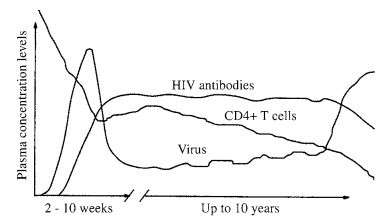
\includegraphics[scale=0.85]{HIV-Infection-Timescale.png}}
	\caption{Schematic time course of a typical HIV infection in an infected adult. The viral concentration, the level of antibodies and the CD4 T-Cells are sketched as a function of time. The early peek represents the primary infection that leads to a period of latency. (From Perelson and Nelson 1999)}
\end{figure}

The level of the virus falls after the initial infection to a level that has been called the set-point. Then, the concentration of the virus seems to remain relatively constant as the CD4 T-cells concentration slowly declines. This period in which the virus concentration is at a quasi-steady state level, while the CD4 T-cells slowly falls, is typically an asymptomatic period, i.e. the person infected does not experience any symptoms that usually would be typical of the disease.\\
Epidemiologists have been puzzled for years about the events that might be happening during the asymptomatic period, until when, in the mid 1990's, became possible to perturb the host-virus system during this period, thanks to the development of new antiretroviral drugs, called protease inhibitors. This drugs block the enzyme protease which HIV uses to  break up large proteins into smaller pieces required to assembly new viral particles. Therefore, in 1994, David Ho, one of the most prominent researchers in the field of HIV treatment, ran an experiment which examined the response of 20 HIV-infected individuals to treatment with ritonavir, a protease inhibitor. The experiment led to dramatic results, with the virus concentration falling rapidly after the ingestion of the drug, as can be seen in figure 1.2.

\begin{figure}[H]
	{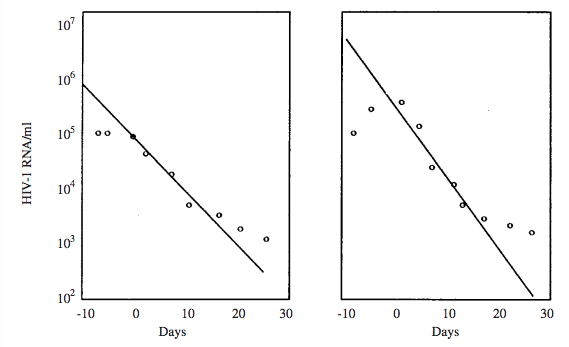
\includegraphics[scale=0.7]{HIV-Protease.png}}
	\caption{After treatment at $t=0$ with ritonavir, the virus concentration declined rapidly. The data are from 2 of the 20 patients studied in Ho et al. (1995), but all 20 patients exhibited similar behavior in the decline of the virus.}
\end{figure}


